\SACCMD{image}
\label{cmd:image}

\SACTitle{概要}
利用内存中的数据文件绘制彩色图

\SACTitle{语法}
\begin{SACSTX}
IMAGE [COLOR|GREY] [BINARY|FULL] [PRINT [pname]]
\end{SACSTX}

\SACTitle{输入}
\begin{description}
\item [COLOR|GREY] 绘制彩图或者灰度图
\item [BINARY|FULL] 绘图时所有正值是一个颜色,所有负值是另一种颜色,或者根据数据值不同变换颜色
\end{description}

\SACTitle{缺省值}
\begin{SACDFT}
image color full
\end{SACDFT}

\SACTitle{说明}
该命令允许用户用SAC三维数据绘制彩图或灰度图。

三维数据可以用 \nameref{cmd:spectrogram}、
\nameref{cmd:sonogram} 或 \nameref{cmd:bbfk} 命令产生,也可以自己生成SAC格式的三维
数据。可以使用 \nameref{cmd:xlim} 和 \nameref{cmd:ylim} 以控制要显示的绘图效果,
也可以使用其他命令对数据做振幅上的操作。

\SACTitle{示例}
以SAC 101.5c自带的contourdata为例:
\begin{SACCode}
SAC> r contourdata
SAC> image
\end{SACCode}

\begin{figure}[!ht]
\centering
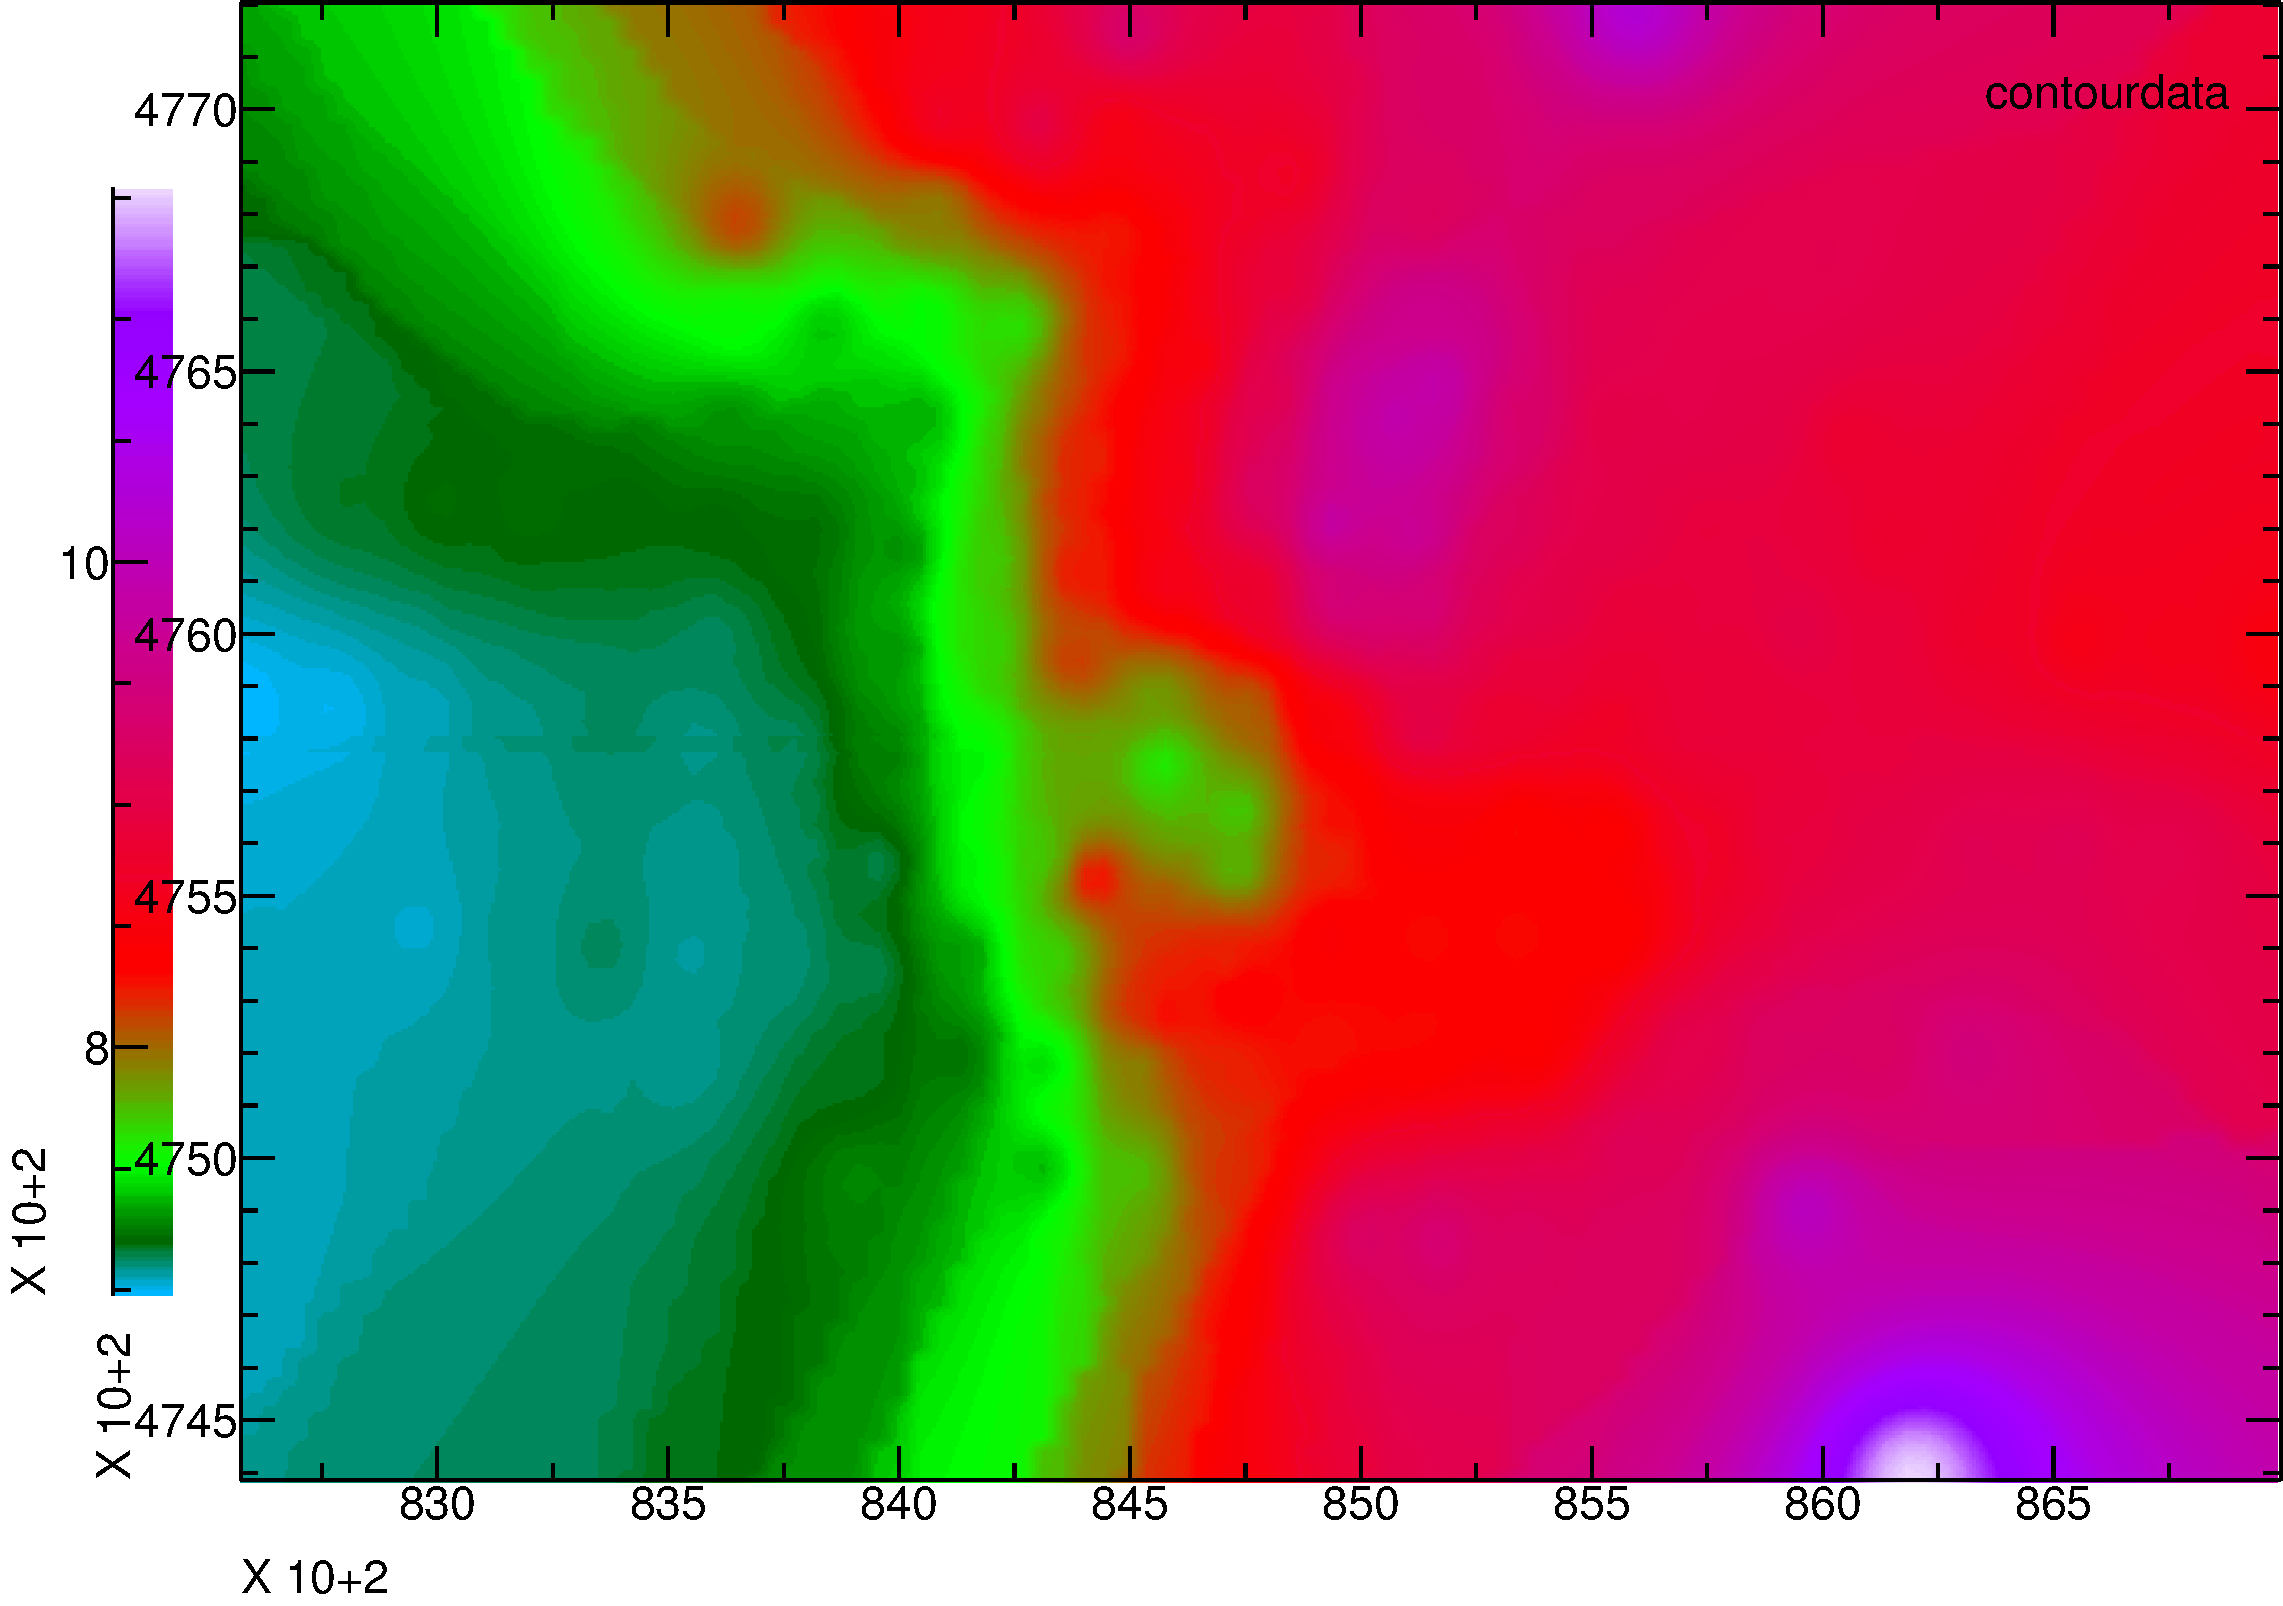
\includegraphics[width=0.9\textwidth]{image}
\caption{image示意图}
\end{figure}

\SACTitle{头段变量}
需要:iftype (设为``IXYZ''), nxsize, nysize

使用:xminimum, xmaximum, yminimum, ymaximum
